\documentclass[programming]{../../../../mfcs}
\newcommand{\projectduedate}{Tuesday, May 9th}
\newcommand{\quarter}{Spring 2017}
\usepackage{color}
\usepackage{multicol}
\usepackage{wrapfig}
\setlength{\belowcaptionskip}{-30pt}
\setlength{\intextsep}{-20pt}
\setlength{\textfloatsep}{0pt}

\course{CSE 154}{Web Programming}{\quarter}
\NoDate
\topic{Homework Assignment 5: Pokedex}
\usepackage{csquotes}
\usepackage{tabularx}

\begin{document}
\vspace{-3.8em}

\hfill\begin{varwidth}{0.5\textwidth}
{\large {\bf\color{colour} Due Date:} \projectduedate}
\end{varwidth}
\vspace{2em}

This assignment is about using \textbf{AJAX} to fetch data in JSON format and process it using DOM
manipulation. 

\newline

\vspace{2em}
\begin{question}{Overview}
In this assignment, you will implement views for a Pokedex and two Pokemon cards.
\textbf{(\emph{Note: You
will not need to know anything about the Pokemon game throughout this assignment, although we hope
you enjoy having a more fun twist to your homework!})} A \textbf{Pokedex} is an encyclopedia (or
album) of different Pokemon species, representing each Pokemon as a small ``sprite'' image. In
this assignment, a Pokedex entry (referenced by the sprite image) will link directly to a
\textbf{Pokemon card}, which is a card of information for a single Pokemon species, containing a
larger image of the Pokemon, its type and
weakness information, its set of moves, health point data, and a short description. 
\newline

  Each Pokemon has one of 18 types (fire, water, grass, normal, electric, fighting, psychic,
  fairy, dark, bug, steel, ice, ghost, poison,
  flying, rock, ground, and dragon) and one weakness type (also from this set of 18 types). Again,
  you don't need to know about the strength/weakness of different types - this information will be
  provided to you as needed.
  \newline
  
  In this assignment, we will simplify things by assuming that each Pokemon has no more than 4 moves (some
  have fewer, but all Pokemon have at least one move). In addition, we assume that the complete
  Pokedex has 151 Pokemon (more have been added over the game's history, but these comprise the original set of Pokemon species).
  \newline
 
  You will create and turn in a JS file called \texttt{\textbf{\color{colour}{pokedex.js}}}.
  This JS file will use the provided \texttt{\textbf{\color{colour}{pokedex.html}}} and \texttt{\textbf{\color{colour}{pokedex.css}}}.
  These HTML and css files are provided with image files in a zipped folder located at
  \newline\texttt{\textbf{\color{colour}{https://webster.cs.washington.edu/pokedex/resources.zip}}}:
\newline

\begin{itemize}
  \item \texttt{\textbf{\color{colour}{pokedex.html}}}: The HTML page for displaying a user's Pokedex and two game cards
\item \texttt{\textbf{\color{colour}{pokedex.css}}}: The style sheet for
  \texttt{\textbf{\color{colour}{pokedex.html}}}
\item \texttt{\textbf{\color{colour}{icons/}}}: \texttt{.jpg} icons for types, weaknesses,
  \texttt{.png} icons for buffs, and \texttt{.gif} icon for loading animation
\item \texttt{\textbf{\color{colour}{images/}}}: \texttt{.jpg} card images for 151 the Pokemon
\item \texttt{\textbf{\color{colour}{sprites/}}}: \texttt{.png} sprite images for 151 the Pokemon
\end{itemize}
\newline

\end{question}
\newpage
\begin{question}{Data}
  You will use JavaScript and AJAX requests to update \texttt{\textbf{\color{colour}{pokedex.html}}} as needed. Your program will
read data from the following two web services we have provided for the assignment:

\begin{itemize}
  \item \texttt{\textbf{\color{colour}{https://webster.cs.washington.edu/pokedex/pokedex.php}}}
  \item \texttt{\textbf{\color{colour}{https://webster.cs.washington.edu/pokedex/game.php}}}
\end{itemize}

We have provided documentation for each of these APIs in \url{hw5-apidoc.pdf}. You will need to
read through this documentation in order to use the APIs properly for this assignment. 
You may assume that the data returned from both of these web services is valid and follows the
formats given.
\newline
\end{question}

\begin{question}{Appearance and Behavior}
  \vspace{0.5em}
\subquestion*{Part I: Main View}
  The provided HTML and CSS files display the main view by default when the page
  is loaded. Below is an example of this template:

  \begin{center}
  \includegraphics[width=0.75\textwidth]{skel-view.png}
  \end{center}

  For the first part of this assignment, you will
  populate the right container (\texttt{\#pokedex-view}) with all 151 Pokemon sprite icons by making an AJAX ``\texttt{GET}'' request to \texttt{pokedex.php?pokedex=all}. You should also initialize your 
  current ``found'' Pokemon in your JS file (you may use a module-global array to do so) with the 
  three starter Pokemon: Bulbasaur, Charmander, and Squirtle. Throughout the game, you will have the 
  chance to collect Pokemon to add to your collection. Below is an image of the expected output (just 
  displaying the \texttt{\#pokedex-view}) when the Pokedex has been populated:
  \newline
  \begin{center}
  \includegraphics[width=0.5\textwidth]{pokedex-view.png}
  \end{center}

  All 151 \texttt{imgs} added to the \texttt{\#pokedex-view} should have a class of
  \texttt{.sprite} and have their \texttt{src} attribute set to the image path returned in the plain
  text response. These image paths will be in the format \texttt{pokemonname.png}. You will need to prepend
  \texttt{sprites/} to the \texttt{src} to correctly link the corresponding sprite
  image (if you are using the images locally, remember to make sure that your
  unzipped image folders are in the same directory as your HTML, CSS, and
  JS files). Initially, the unfound Pokemon should have the additional class \texttt{.unfound}. 
  These Pokemon sprites will show up as black shadows with this class as opposed to the colored
  versions without.
  \newline

  For each ``found'' sprite added to the \texttt{\#pokedex-view}, you will need to add an event handler so
  that when the sprite is clicked, the card on the left is populated with that Pokemon's data. You
  will retrieve this data using the \texttt{pokedex.php?pokemon=parameter} request, passing the clicked
  Pokemon's name as the parameter (you may find it helpful to give each sprite an id with the
  Pokemon's name). If a Pokemon with the class \texttt{.unfound} is
  clicked, nothing should happen.
  \newline

  \subquestion*{Card View}
    \begin{wrapfigure}{h}{0.32\textwidth}
    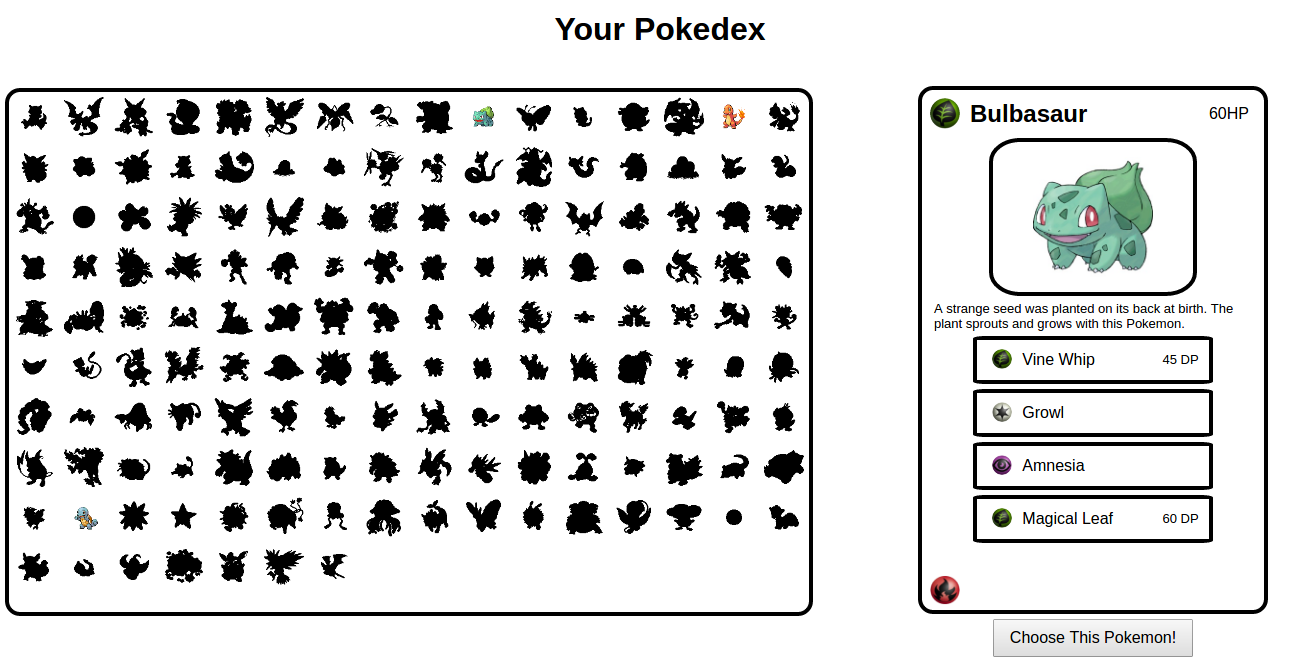
\includegraphics[width=0.32\textwidth]{bulbasaur-card.png}
    \end{wrapfigure}
  Once a found Pokemon is clicked, the card data for that Pokemon populates the card on the left
  side of the page. This card has the id of \texttt{\#my-card}. You should use the returned JSON
  object from the \texttt{pokedex?pokemon=parameter} request to populate the card with the Pokemon's
  information, as explained below:
  \begin{itemize}
    \item The ``\texttt{name}'' value should populate the \texttt{\#my-card .name} heading with the
      name of the Pokemon. 
    \item The ``\texttt{images}'' value is a collection of three folder paths, the first being
      ``\texttt{photo}'' to link to the Pokemon's photo (referenced by \texttt{\#my-card .pokepic}), the second being ``\texttt{typeIcon}'' to link to the
      type icon of the Pokemon in the top-left corner (\texttt{\#my-card .type}), and the third being the ``\texttt{weaknessIcon}'' to link to the weakness
      type icon of the Pokemon in the bottom-left corner (\texttt{\#my-card
      .weakness}).
    \item The ``\texttt{hp}'', or health point value should populate the \texttt{\#my-card .hp} span positioned at the top-right corner of the card. You will need to append ``HP'' to
      the provided hp value, as shown in the example card image to the right.
  \end{itemize}

  \begin{itemize}
    \item The ``\texttt{description}'' attribute should be used to populate the card with the Pokemon's
      description. The description should be placed in the provided \texttt{\#my-card .info} div.
    \item The ``\texttt{moves}'' attribute includes data about the Pokemon's moves (between 1 and 4 moves,
      depending on the Pokemon). You should populate only enough move buttons in
      \texttt{\#my-card .moves} for the Pokemon's move count. If there are fewer than four moves
      for a Pokemon, you should set the extra buttons to have the class of \texttt{.hidden} so that
      they do not display visible on the card for that Pokemon. Any hidden moves should
      be below the visible moves in the \texttt{.moves div}.  Each move button should have its \texttt{innerText} set to the provided move name, and its
      corresponding \texttt{img} icon set to have a \texttt{src} attribute of that move's type
      (similar to how you did the type and weakness for the Pokemon). These type images will show to
      the left of the move's name. The order of moves appended to a card does not matter, but you
      may find it easiest to populate them based on the order they are returned in the moves array.
  \end{itemize}

  Finally, you should make visible the \texttt{\#start-btn} once a user has clicked any of their
  discovered Pokemon. In other words, the button should not be visible until the card is populated
  with a Pokemon's information.
\newpage
\subquestion*{Part II: Game View}
  Clicking the ``Choose This Pokemon'' button under the Pokemon card view should hide the \texttt{\#pokedex-view} and show the
  second player's card, \texttt{\#their-card}, resulting in the view similar to that below (where
  ``your'' Pokemon is chosen as Bulbasaur, and the opponent's Pokemon is Ditto). You should also
  make the \texttt{\#results-container div} visible at this point, which will populate the center of the page with turn
  results for each move made.
  \newline

  \vspace{0.5em}
  \includegraphics[width=\textwidth]{turn-results.png}
  \newline
  To initialize the game, you will need to make a \texttt{POST}
  request to \texttt{game.php} with the \texttt{POST} parameters of \texttt{startgame=true} and
  \texttt{mypokemon=yourpokemonsname}. This request will return the initial game state, including
  data for your card and data for the opponent's card. This request will also return unique
  \texttt{guid} (game ID) and \texttt{pid} (player ID) values that you should store as module-global variables in your
  file. These values will be necessary to play moves during the game. You will use this data to populate each card
  with image, stats, and move data for each Pokemon. Note that you already should have the necessary
  data populated in your card, so won't necessarily need to re-populate at this point. You will need
  to display your cards hidden \texttt{.buffs div} though for visibility during the game, and make
  sure that your opponent's card also has their \texttt{.buffs div} visible (both will initially
  start with no buffs). Your
  opponent's card will be given as a random Pokemon (in the example output image above, the random
  Pokemon is called Ditto), and should be populated with the data similar to how you populated your card on the
  previous step. Note that there is quite a bit of redundancy here, so you should factor out
  redundant DOM manipulation code as much as possible.
  \newline

\textbf{Game Play:}
Each move that you make has an effect on the game state which is handled by the server. All you need
to do to keep track of the game state is update the game with the data returned by the
\texttt{game.php} play move \texttt{POST} request.
You should make this request whenever a user
clicks on \emph{their} Pokemon's moves, and remove the \texttt{.hidden} class from the
\texttt{\#loading} image to display a loading animation while the request is being processed. 
Once the request responds with the data successfully, this animation should become hidden again. The returned game data includes a \texttt{results} array
that provides the results of both Pokemon's moves (which moves were played and whether they were a hit or miss) and you should
display these in the \texttt{\#p1-turn-results} and \texttt{\#p2-turn-results divs} in the
\texttt{\#turn-results div} in the center of the page, as shown in the above example.
\newpage

There are a few changes 
that may result from the updated game
state, each of which you need to handle:

\begin{itemize}
  \item \textbf{Damage is dealt to your Pokemon and/or the opponent's Pokemon}: The returned game
    state provides data about the current health of both Pokemon. You should update the health bar
    (the \texttt{.health-bar div} on each card) to make its width a percentage of the max width, where
    the percentage is calculated as \texttt{current-hp / hp} using these values from the returned
    JSON. If the percentage is less than 20\%, the health-bar should have a class of
    \texttt{.low-health} added to make it red (see image above for an example). When the health is greater than or equal to 20\% of
    the total health, it should never have a \texttt{.low-health} class (Pokemon may have healing
    moves, so you should remove this class if they're health rises above 20\% after having low
    health).
  \item \textbf{Buffs}:
    Some Pokemon have moves that apply ``buffs'' or ``debuffs'' to themselves or the opponent Pokemon.
    In this case, you will need to add or remove divs to each card's \texttt{.buffs div}. There are three
    stats that may have buffs applied: attack, defense, and accuracy. Attack buffs \texttt{.attack} are represented
    as red arrows, defense buffs \texttt{.defense} are represented as blue arrows, and accuracy
    buffs \texttt{.accuracy} are represented
    as green arrows. Helpful buffs are arrows pointed upwards (with the \texttt{.buff} class) and 
    harmful buffs are arrows pointed downwards (with the \texttt{.debuff} class). The returned game
    state for each Pokemon has a \texttt{buffs} and \texttt{debuffs} array with the number of stats
    for each listed as string values (see the API documentation).
\end{itemize}

\textbf{Winning/Losing:} The game ends when one of the Pokemon has 0 hp points. You should append a
message in the \texttt{\#title} as ``You won!'' or ``You lost!'' depending on the results of
the game and then remove the \texttt{.hidden} class to \texttt{\#endgame}. 
Below is an example output after you have won the game:
\begin{center}
  \includegraphics[width=\textwidth]{resultsv2.png}
\end{center}
\newline

The  \texttt{\#endgame}
button will appear in the center of the page when visible, just under the \texttt{\#title}. You
should display \texttt{\#p1-turn-results} with the data populated in \texttt{\#p1-move} and
\texttt{\#p1-result}, but if you were the last one to make a move (e.g., your move causes P2's HP to
go to 0 before they make a move),
\texttt{\#p2-result} and \texttt{\#p2-move} will be returned as empty strings. If this is the case,
you should not display any message for P2's move for this final turn in this case. 
\newline

When clicked, the \texttt{\#endgame} button should switch back to the Pokedex View and then become hidden again. 
Whatever Pokemon you chose most-recently should populate \texttt{\#my-card}, in case the user wants to use
that Pokemon again for a subsequent game. \texttt{\#start-btn} should also be re-displayed after
switching to the Pokedex view at this point, and the \texttt{\#results-container} should also be
hidden. 
\newline

If you win the game and the opponent has a Pokemon that you have
not found, you may add it to your Pokedex by adding it to your collection of found Pokemon (e.g., a
module-global array of Pokemon, which started with Bulbasaur, Charmander, and Squirtle). You should
then remove the \texttt{.unfound} class from the associated Pokemon and add an onclick handler to
allow it to be chosen for another game (similar to how you did with
the three starter Pokemon).
\newline

\textbf{Fleeing:}
There is a button under your card during the game labeled ``Flee the Battle''. If clicked, this
  should make a POST request to \texttt{game.php} with parameters \texttt{move=flee},
  \texttt{guid=yourguid}, and \texttt{pid=yourpid}, where the \texttt{guid} and \texttt{pid} are
  your unique game and player id values. This request will terminate your game
  and declare your opponent as the winner by automatically setting your HP to 0. You should display
  a message as described in the "lose case" above when your receive the response to playing this
  move. Note that your Pokemon will flee immediately before the second player makes a move, so they
  will not have any move results returned (you should not display any results for Player 2, just
  your flee move results).
\end{question}

\begin{question}{Implementation and Grading}
Separate content (HTML), presentation (CSS), and behavior (JavaScript).
Your JavaScript code should use styles and classes from the CSS provided rather than manually
setting each style property in the JavaScript. The provided CSS file should have all of the classes required to
  achieve the desired output. 
\newline

Your JavaScript code should pass our JSLint tool with no errors. Your \texttt{.js} file must run in
  strict mode by putting \texttt{"use strict";} within your module.
Capture common operations as functions to keep code size and complexity from growing. You can reduce your code size by using the \texttt{this} keyword in your event handlers.
\newline

No global variables or functions are allowed. To avoid globals, use the module pattern as taught in lecture,
wrapping your code in an anonymous function invocation. Even if you use the module pattern, limit the amount of
  ``module-global'' variables to those that are truly necessary (we have given suggestions about
  those that you will need); values should be local as much as
  possible. If a particular
      literal value is used frequently, declare it as a module-global ``constant'' variable
      \texttt{IN\_UPPER\_CASE} and use the
constant in your code.
\newline

Do not store DOM element objects, such as those returned by
\texttt{document.getElementById} or \texttt{document.querySelectorAll}, as module-global variables. 
\newline

Your JavaScript code should follow the style guide and should have adequate commenting. The top of your
JavaScript file should have a descriptive
comment header describing the assignment, and each function and complex section of code should be documented.
Format your code similarly to the examples from class. Properly use whitespace and indentation. Use good
variable and method names. Avoid lines of code more than 100 characters wide. For reference, our \texttt{.js} file has
  roughly 180 lines (120 ``substantive'').
\newline

Do not place your solution on a public web site. Submit your own work and follow the course misconduct policy.
\end{question}
\end{document}
